% =====================================================================
% CardShark-RL — IEEE Two-Column Paper
% CENG 454 Final Project Report
% =====================================================================
\documentclass[conference]{IEEEtran}

\IEEEoverridecommandlockouts

\usepackage{cite}
\usepackage{amsmath,amssymb,amsfonts}
\usepackage{algorithmic}
\usepackage{graphicx}
\usepackage{textcomp}
\usepackage{xcolor}
\usepackage{booktabs}
\usepackage{url}
\usepackage{hyperref}
\usepackage{multirow}
\usepackage{array}

\graphicspath{{../latest results/}}

\hypersetup{
    colorlinks=true,
    linkcolor=blue,
    citecolor=blue,
    urlcolor=blue
}

\def\BibTeX{{\rm B\kern-.05em{\sc i\kern-.025em b}\kern-.08em
    T\kern-.1667em\lower.7ex\hbox{E}\kern-.125emX}}

% =====================================================================
\begin{document}

\title{Decoding ``The Tell'': Exploitative Reinforcement Learning\\
and Implicit Opponent Modeling in 5-Card Draw Poker}

\author{
  \IEEEauthorblockN{[Author Names]}
  \IEEEauthorblockA{
    \textit{Department of Computer Engineering}\\
    \textit{Izmir Katip Celebi University}\\
    Izmir, Turkey
  }
}

\maketitle

% =====================================================================
\begin{abstract}
Poker is a canonical benchmark for artificial intelligence research in
imperfect-information games, requiring agents to reason under
uncertainty, manage hidden state, and adapt strategy to diverse
opponents. This paper presents \textbf{CardShark-RL}, a reinforcement
learning system for heads-up limit 5-Card Draw Poker that investigates
two complementary approaches to opponent adaptation: (A) explicit
opponent modeling, in which a one-hot identifier encodes the opponent
archetype directly in the observation, and (B) implicit opponent
modeling, in which the agent infers opponent behavior from a rolling
window of behavioral statistics. Both agents are trained using
MaskablePPO \cite{raffin2021stable} within a custom PettingZoo
\cite{terry2021pettingzoo} environment. We further apply Optuna-based
hyperparameter optimization \cite{akiba2019optuna} and reward shaping
to improve convergence. The two models are evaluated against three
hand-crafted opponent archetypes---Calling Station, Maniac, and
Rock---over 10,000 hands each. We analyze ``The Tell'': the behavioral
signature that Model~B learns to exploit based solely on an opponent's
draw-count pattern, without access to any explicit opponent identity.
Our results show that Model~B (Implicit) achieves +166.50 BB/100 on
average across all archetypes, compared to +180.65 BB/100 for Model~A
(Explicit), a gap that is statistically significant ($p = 0.029$) yet
practically modest, and that Model~B outperforms an oracle-labeled
explicit agent in a non-stationary setting (+160.35 vs.\ +156.28 BB/100).
\end{abstract}

\begin{IEEEkeywords}
reinforcement learning, opponent modeling, poker AI, MaskablePPO,
imperfect-information games, reward shaping, behavioral inference,
hyperparameter optimization
\end{IEEEkeywords}

% =====================================================================
\section{Introduction and Motivation}
\label{sec:intro}

Poker has long served as a proving ground for AI research on
decision-making under uncertainty. Unlike chess or Go, poker involves
hidden information---players observe only their own cards and the
shared betting history---creating a setting where an optimal strategy
must reason about the probability distributions over unobserved states
and simultaneously adapt to the behavioral tendencies of the opponent.
This combination of imperfect information, sequential decision-making,
and strategic adaptation makes poker a rich and challenging domain for
reinforcement learning (RL).

Landmark systems such as Libratus \cite{brown2018libratus}, DeepStack
\cite{moravcik2017deepstack}, and Pluribus \cite{brown2019superhuman}
have achieved superhuman performance in Texas Hold'em by combining
Counterfactual Regret Minimization (CFR) \cite{zinkevich2007regret}
with sophisticated endgame solving. While these systems represent the
state of the art in game-theoretically optimal play, they are
computationally expensive, require large-scale game-tree traversal,
and are primarily designed to resist exploitation rather than to
actively exploit opponent weaknesses.

In contrast, this work investigates \textit{exploitative} RL:
training a deep policy network to identify and profit from specific,
predictable patterns in opponent behavior. We focus on 5-Card Draw
Poker, a historically significant variant that has received less
attention in the modern deep learning era, and we formulate a concrete
research question: \textit{Can a reinforcement learning agent
adaptively exploit behaviorally distinct opponents through implicit
modeling alone, without access to explicit opponent identity
information?}

To answer this question, we design and implement \textbf{CardShark-RL},
a complete RL training and evaluation pipeline featuring:
\begin{itemize}
    \item A custom PettingZoo AEC environment for limit heads-up
    5-Card Draw Poker with three hard-coded opponent archetypes;
    \item \textbf{Model~A} (Explicit): a MaskablePPO agent that
    receives a one-hot encoding of the opponent archetype in its
    observation vector;
    \item \textbf{Model~B} (Implicit): a MaskablePPO agent that
    receives only a rolling window of 10 behavioral statistics computed
    from past hands, with no direct opponent identity signal;
    \item Optuna-based hyperparameter optimization with a
    Rock-weighted objective function;
    \item Reward shaping to encourage aggressive exploitation;
    \item A behavioral matrix analysis, ``The Tell'', that reveals
    how Model~B adapts its post-draw betting strategy based on
    opponent draw counts.
\end{itemize}

The remainder of this paper is organized as follows.
Section~\ref{sec:related} reviews related work. Section~\ref{sec:env}
describes the game environment and opponent archetypes.
Section~\ref{sec:method} details the proposed methodology.
Sections~\ref{sec:results}--\ref{sec:conclusion} present results,
discussion, and conclusions.

% =====================================================================
\section{Background and Related Work}
\label{sec:related}

\subsection{Game-Theoretic Poker AI}

The challenge of building superhuman poker AI has driven decades of
research. Early milestones include Polaris \cite{zinkevich2007regret},
which applied CFR variants to limit Texas Hold'em. The breakthrough
work of Libratus \cite{brown2018libratus} achieved superhuman
performance in heads-up no-limit Texas Hold'em in 2017 using an
endgame solver and safe subgame-refinement techniques \cite{ganzfried2015endgame}.
DeepStack \cite{moravcik2017deepstack} concurrently demonstrated that
deep neural networks could replace the look-up tables used in
endgame solving, enabling real-time play without pre-computed
strategies. Pluribus \cite{brown2019superhuman} subsequently extended
this paradigm to six-player no-limit Hold'em, the first superhuman
AI to master multiplayer poker. A key distinction of these systems is
their focus on \textit{equilibrium strategies}---policies robust to
any opponent---rather than \textit{exploitative} strategies that
target specific opponent weaknesses.

\subsection{Deep Reinforcement Learning in Games}

Deep reinforcement learning has achieved remarkable results in a wide
range of games. Mnih et al.~\cite{mnih2015human} demonstrated that
DQN could achieve human-level performance on Atari games by combining
Q-learning with deep convolutional networks, experience replay, and
target networks. Silver et al.~\cite{silver2016mastering} applied
deep RL and Monte Carlo tree search to master the game of Go, a
domain previously thought intractable for AI. The Proximal Policy
Optimization (PPO) algorithm \cite{schulman2017proximal}, introduced
by Schulman et al., provides a stable and sample-efficient policy
gradient method well-suited to discrete action environments such as
card games. PPO's clipped surrogate objective prevents destructively
large policy updates while remaining simpler to implement than its
predecessor, TRPO. In our work, we use MaskablePPO, an extension of
PPO from the sb3-contrib library \cite{raffin2021stable}, which
incorporates action masking to handle the structured invalid-action
spaces that arise in poker (betting during draw phases and vice versa).

\subsection{Action Masking in Reinforcement Learning}

Huang and Onta\~{n}{\'o}n~\cite{huang2022closer} provide a
theoretical and empirical analysis of invalid action masking in policy
gradient algorithms. They demonstrate that masking is critical when
the ratio of invalid to valid actions is large, as penalty-based
approaches fail to learn in such settings. In 5-Card Draw Poker,
the agent faces a discrete action space of 35 actions (Fold, Call,
Raise, and 32 draw bitmask combinations), of which only a small
subset is legal at any given game state. Action masking is therefore
essential for efficient learning and training stability.

\subsection{Opponent Modeling and Behavioral Inference}

Opponent modeling in multi-agent settings has been studied
extensively, with approaches ranging from Bayesian inference over
opponent type distributions to neural network-based latent
representations. Explicit modeling approaches
build a dedicated representation of the opponent (e.g., type
classification or hand-range estimation), while implicit approaches
allow the agent's policy to adapt to opponent behavior through
reward-maximizing experience without an explicit opponent model. The
rolling-statistics approach employed by Model~B, tracking metrics
such as VPIP (Voluntarily Put In Pot), Pre-draw Raise frequency, and
Aggression Factor, aligns with the behavioral profiling tradition in
poker theory and has parallels with the latent opponent-embedding
approaches studied in recent deep multi-agent RL literature.

\subsection{Hyperparameter Optimization}

Hyperparameter optimization (HPO) is critical for RL systems, where
training outcomes are sensitive to learning rates, architecture
choices, and exploration-exploitation trade-offs. Akiba et
al.~\cite{akiba2019optuna} introduced Optuna, a next-generation HPO
framework using tree-structured Parzen estimators (TPE) for efficient
Bayesian search. We employ Optuna's MedianPruner with warm-up steps
to prune underperforming trials early, enabling efficient search over
a 15-dimensional hyperparameter space.

\subsection{Reward Shaping}

Ng et al.~\cite{ng1999policy} established the theoretical foundation
for potential-based reward shaping, proving that shaped rewards
preserve the set of optimal policies under suitable conditions. In
poker, raw chip profit is a natural but sparse reward signal. We
introduce two auxiliary shaping terms---a penalty for folding when
checking was available, and a bonus for successful steal attempts---to
guide the agent toward more aggressive exploitation strategies.

% =====================================================================
\section{Environment Design}
\label{sec:env}

\subsection{5-Card Draw Poker Rules}

CardShark-RL implements limit heads-up 5-Card Draw Poker, a
two-player variant in which each player is dealt five private cards
and proceeds through four phases:
\begin{enumerate}
    \item \textbf{Antes}: Both players post a forced bet of 1 chip.
    \item \textbf{Pre-draw betting}: A round of limit betting using
    a small bet of 2 chips, with up to 4 raises.
    \item \textbf{Draw phase}: Each player selects 0--5 cards to
    discard and receives replacements from the deck.
    \item \textbf{Post-draw betting}: A final round of betting using
    a big bet of 4 chips, with up to 4 raises.
    \item \textbf{Showdown}: The player with the best 5-card hand
    wins the pot.
\end{enumerate}

A player may win before showdown by causing the opponent to fold.

\subsection{PettingZoo AEC Environment}

The game is implemented as a PettingZoo Agent-Environment Cycle (AEC)
environment \cite{terry2021pettingzoo}, a standardized API for
turn-based multi-agent systems. The AEC model alternates agent turns
in a well-defined cycle, making it natural for sequential card games.
The environment is wrapped by a Gymnasium-compatible
\cite{brockman2016openai} single-agent wrapper (\texttt{DrawPokerGymEnv})
that auto-steps the opponent, presenting the RL agent
(\texttt{player\_0}) with a standard \texttt{(obs, reward, done,
info)} interface.

\subsection{Action Space}

The action space is \texttt{Discrete(35)}:
\begin{itemize}
    \item \textbf{Action 0}: Fold
    \item \textbf{Action 1}: Call / Check
    \item \textbf{Action 2}: Raise / Bet
    \item \textbf{Actions 3--34}: Draw actions, where the index
    encodes a 5-bit bitmask over the five card positions
    (bit $i = 1$ discards card~$i$). Action~3 corresponds to
    bitmask~0 (stand pat; discard nothing), and Action~34
    corresponds to bitmask~31 (discard all five cards).
\end{itemize}

An action mask vector of 35 binary flags is maintained at each
step, enabling MaskablePPO \cite{huang2022closer} to restrict the
policy to legal actions. During betting phases, only Actions 0--2
are legal; during the draw phase, only Actions 3--34 are legal.

\subsection{Observation Space}

The observation vector is a 26-dimensional (for Model~A) or
33-dimensional (for Model~B) float32 array normalized to $[0,1]$
(or $[-1,1]$ for opponent-draw features). The core 23 features
shared by both models are:

\begin{itemize}
    \item \textbf{Hand encoding} (10 features): For each of the
    five cards, a normalized rank $\in [0,1]$ and normalized suit
    $\in [0,1]$.
    \item \textbf{Hand strength} (2 features): Normalized hand
    category (0=High Card to 8=Straight Flush) and normalized
    evaluation score.
    \item \textbf{Pot features} (3 features): Normalized pot size,
    normalized bet-to-call, and pot odds ratio.
    \item \textbf{Phase encoding} (3 features): One-hot vector
    $\in \{$pre-draw, draw, post-draw$\}$.
    \item \textbf{Opponent draw count} (1 feature): Normalized
    number of cards the opponent drew, or $-1$ if the draw phase
    has not yet occurred.
    \item \textbf{Strategic features} (4 features): Positional
    indicator (in/out of position), own raise count (normalized),
    opponent aggression flag, and opponent pre-draw raise flag.
\end{itemize}

\textbf{Model~A} appends a 3-dimensional one-hot vector encoding
the opponent archetype (Calling Station, Maniac, or Rock).

\textbf{Model~B} appends a 10-dimensional rolling statistics vector
computed over the last $W$ hands:
\begin{enumerate}
    \item Fold frequency pre-draw
    \item Fold frequency post-draw
    \item Raise frequency post-draw
    \item Average cards drawn (normalized)
    \item Raise-then-stand-pat correlation
    \item Fold-after-drawing-3 frequency
    \item Raise-after-standing-pat frequency
    \item VPIP (Voluntarily Put In Pot)
    \item PFR (Pre-draw Raise frequency)
    \item Aggression Factor (raises / calls, normalized)
\end{enumerate}

\subsection{Hand Evaluator}

Cards are encoded as integers $0$--$51$ where $\text{rank} = c
\bmod 13$ (0=2, \ldots, 12=A) and $\text{suit} = \lfloor c / 13
\rfloor$ (0=Clubs, \ldots, 3=Spades). Hand evaluation returns a
scalar score $= \text{category} \times 10^6 + \text{tiebreaker}$,
where the tiebreaker uses base-14 encoding of rank groups, ensuring
score ordering within and across all nine hand categories (High Card
through Straight Flush).

\subsection{Opponent Archetypes}

Three hand-crafted deterministic/stochastic opponents model
behaviorally distinct playing styles:

\textbf{CallingStation} (Archetype~0): A passive opponent that never
bluffs and never raises. It always calls and draws optimally by
keeping its best group (pair, trips, etc.) and discarding kickers.

\textbf{Maniac} (Archetype~1): An aggressive opponent that raises
70\% of the time when raising is legal, and chases flush and straight
draws 60\% of the time during the draw phase by drawing one card.
It rarely folds (5\% probability), creating a loose, unpredictable style.

\textbf{Rock} (Archetype~2): A tight-passive opponent that folds
pre-draw on all unpaired hands if there is a bet to call, calls only
with a pair below Jacks, raises with Jacks-or-better, and stands pat
on two-pair or better hands. This opponent is the hardest to exploit,
as it only invests chips with strong holdings.

% =====================================================================
\section{Methodology}
\label{sec:method}

\subsection{Training Algorithm: MaskablePPO}

Both models are trained using MaskablePPO from sb3-contrib
\cite{raffin2021stable}, a variant of Proximal Policy Optimization
\cite{schulman2017proximal} that incorporates action masking directly
into the policy gradient update. The policy is an MLP
(Multi-Layer Perceptron) actor-critic network. The clipped
surrogate objective of PPO is:

\begin{equation}
\mathcal{L}^{\text{CLIP}}(\theta) = \hat{\mathbb{E}}_t \left[
  \min\!\left( r_t(\theta)\hat{A}_t,\;
  \text{clip}(r_t(\theta), 1-\epsilon, 1+\epsilon)\hat{A}_t \right)
\right]
\label{eq:ppo}
\end{equation}

where $r_t(\theta) = \pi_\theta(a_t|s_t) / \pi_{\theta_\text{old}}
(a_t|s_t)$ is the probability ratio and $\hat{A}_t$ is the
Generalized Advantage Estimate (GAE) \cite{schulman2016high}. The
GAE with parameter $\lambda$ interpolates between one-step TD error
($\lambda=0$) and Monte Carlo returns ($\lambda=1$):

\begin{equation}
\hat{A}_t = \sum_{l=0}^{\infty} (\gamma\lambda)^l \delta_{t+l},
\quad \delta_t = r_t + \gamma V(s_{t+1}) - V(s_t)
\label{eq:gae}
\end{equation}

Action masking is applied at inference time by setting the
log-probabilities of illegal actions to $-\infty$ before the
softmax, ensuring the agent never samples illegal actions.
Huang and Onta\~{n}{\'o}n~\cite{huang2022closer} demonstrate that
this hard masking is both theoretically sound and empirically
superior to penalty-based alternatives.

\subsection{Network Architecture}

Both models use an MLP policy with fully connected layers of
equal width. The policy and value networks share no parameters;
each is a separate MLP head on top of the shared feature extractor.
For Model~B (implicit), the optimized architecture uses four hidden
layers of 256 neurons each (depth chosen by HPO). For Model~A
(explicit), a three-layer architecture of 256 neurons is used as the
default.

\subsection{Reward Function}

The base reward at the end of each hand is the net chip profit:
$r = \text{pot\_won} - \text{chips\_invested}$ for the winner, and
$r = -\text{chips\_invested}$ for the loser. Ties yield $r=0$.

Two shaping terms \cite{ng1999policy} are added:
\begin{itemize}
    \item \textbf{Fold penalty} $(-\alpha)$: Applied when the agent
    folds during a phase in which checking would have been free
    (bet-to-call = 0). This penalizes unnecessarily surrendering
    equity.
    \item \textbf{Steal bonus} $(+\beta)$: Applied when the agent
    raises and the opponent subsequently folds (a successful steal).
    This rewards aggressive pot-theft.
\end{itemize}

The shaping weights $\alpha$ and $\beta$ are treated as
hyperparameters and tuned by Optuna. For Model~B, the optimized
values are $\alpha = 0.296$ and $\beta = 0.448$.

\subsection{Opponent Scheduling}

For Model~A (explicit), random opponent scheduling is used:
a new archetype is chosen uniformly at random before each episode.
Since the agent has direct access to the opponent's identity through
the one-hot feature, it can immediately condition its policy on the
current archetype.

For Model~B (implicit), a \textit{hybrid schedule} is employed. The
first $H$ episodes use \textit{block scheduling}: opponents are
cycled through in blocks of $B$ consecutive hands, allowing the
rolling statistics to build up a stable behavioral signal before the
agent can exploit it. After $H$ episodes, random scheduling is
resumed to encourage robustness. The switch point $H$ and block size
$B$ are chosen by HPO.

\subsection{Hyperparameter Optimization with Optuna}

We employ Optuna \cite{akiba2019optuna} with Tree-structured Parzen Estimator (TPE) sampling and a MedianPruner to search over a 15-dimensional hyperparameter space. The best configurations found for both models are summarized in Table~\ref{tab:best_params}. Each trial trains the model for 300,000 timesteps and is evaluated using a Rock-weighted objective:
\begin{equation}
\text{score} = 0.5 \cdot \text{BB}_{100}^{\text{Rock}}
             + 0.25 \cdot \text{BB}_{100}^{\text{Station}}
             + 0.25 \cdot \text{BB}_{100}^{\text{Maniac}}
\label{eq:hpo_obj}
\end{equation}

The Rock archetype receives extra weight (0.5) because it is the
hardest opponent to exploit and determines whether the agent has
learned genuine strategic depth or is merely farming easy wins
against passive opponents.

\begin{table}[htbp]
\caption{Best Hyperparameters for Model A (Explicit) and Model B (Implicit)}
\label{tab:best_params}
\centering
\begin{tabular}{lll}
\toprule
\textbf{Hyperparameter} & \textbf{Model A (Explicit)} & \textbf{Model B (Implicit)} \\
\midrule
learning\_rate      & $1.63 \times 10^{-4}$ & $3.50 \times 10^{-4}$ \\
n\_steps            & 4096 & 2048 \\
batch\_size         & 32 & 64 \\
n\_epochs           & 22 & 11 \\
gamma               & 0.9658 & 0.9894 \\
ent\_coef           & 0.00103 & 0.00457 \\
clip\_range         & 0.242 & 0.194 \\
gae\_lambda         & 0.874 & 0.922 \\
vf\_coef            & 0.475 & 0.430 \\
max\_grad\_norm     & 0.484 & 0.464 \\
fold\_penalty       & 0.379 & 0.328 \\
steal\_bonus        & 0.492 & 0.212 \\
lr\_schedule        & constant & linear \\
net\_arch           & [128, 128] & [256, 256, 256, 256] \\
rolling\_window $W$ & N/A & 50 \\
block\_size $B$     & N/A & 400 \\
hybrid\_switch $H$  & N/A & 972{,}000 steps \\
\bottomrule
\end{tabular}
\end{table}

\subsection{Training Protocol}

Both models are trained for 1{,}000{,}000 timesteps using
$n_\text{envs} = 4$ parallel environments (DummyVecEnv) with
distinct random seeds. A per-opponent evaluation callback runs every
50{,}000 timesteps, reporting intermediate BB/100 values for each
archetype to monitor learning dynamics. Training is performed on a
single machine; the device is selected automatically (CPU or CUDA).

\subsection{Evaluation Metric: BB/100}

Performance is reported in \textit{big blinds per 100 hands}
(BB/100), a standard poker metric:
\begin{equation}
\text{BB/100} = \frac{\text{total profit}}{\text{number of hands}} \times 100
\label{eq:bb100}
\end{equation}

where the big blind equals 4 chips (the post-draw bet size) in
our game. A positive BB/100 indicates a profitable strategy; a
negative value indicates a losing strategy. Each evaluation run
uses 10{,}000 hands against a fixed opponent archetype with a warm-up
phase of 50 random hands (for Model~B only) to populate the rolling
statistics buffer before evaluation begins.

\begin{figure}[htbp]
  \centering
  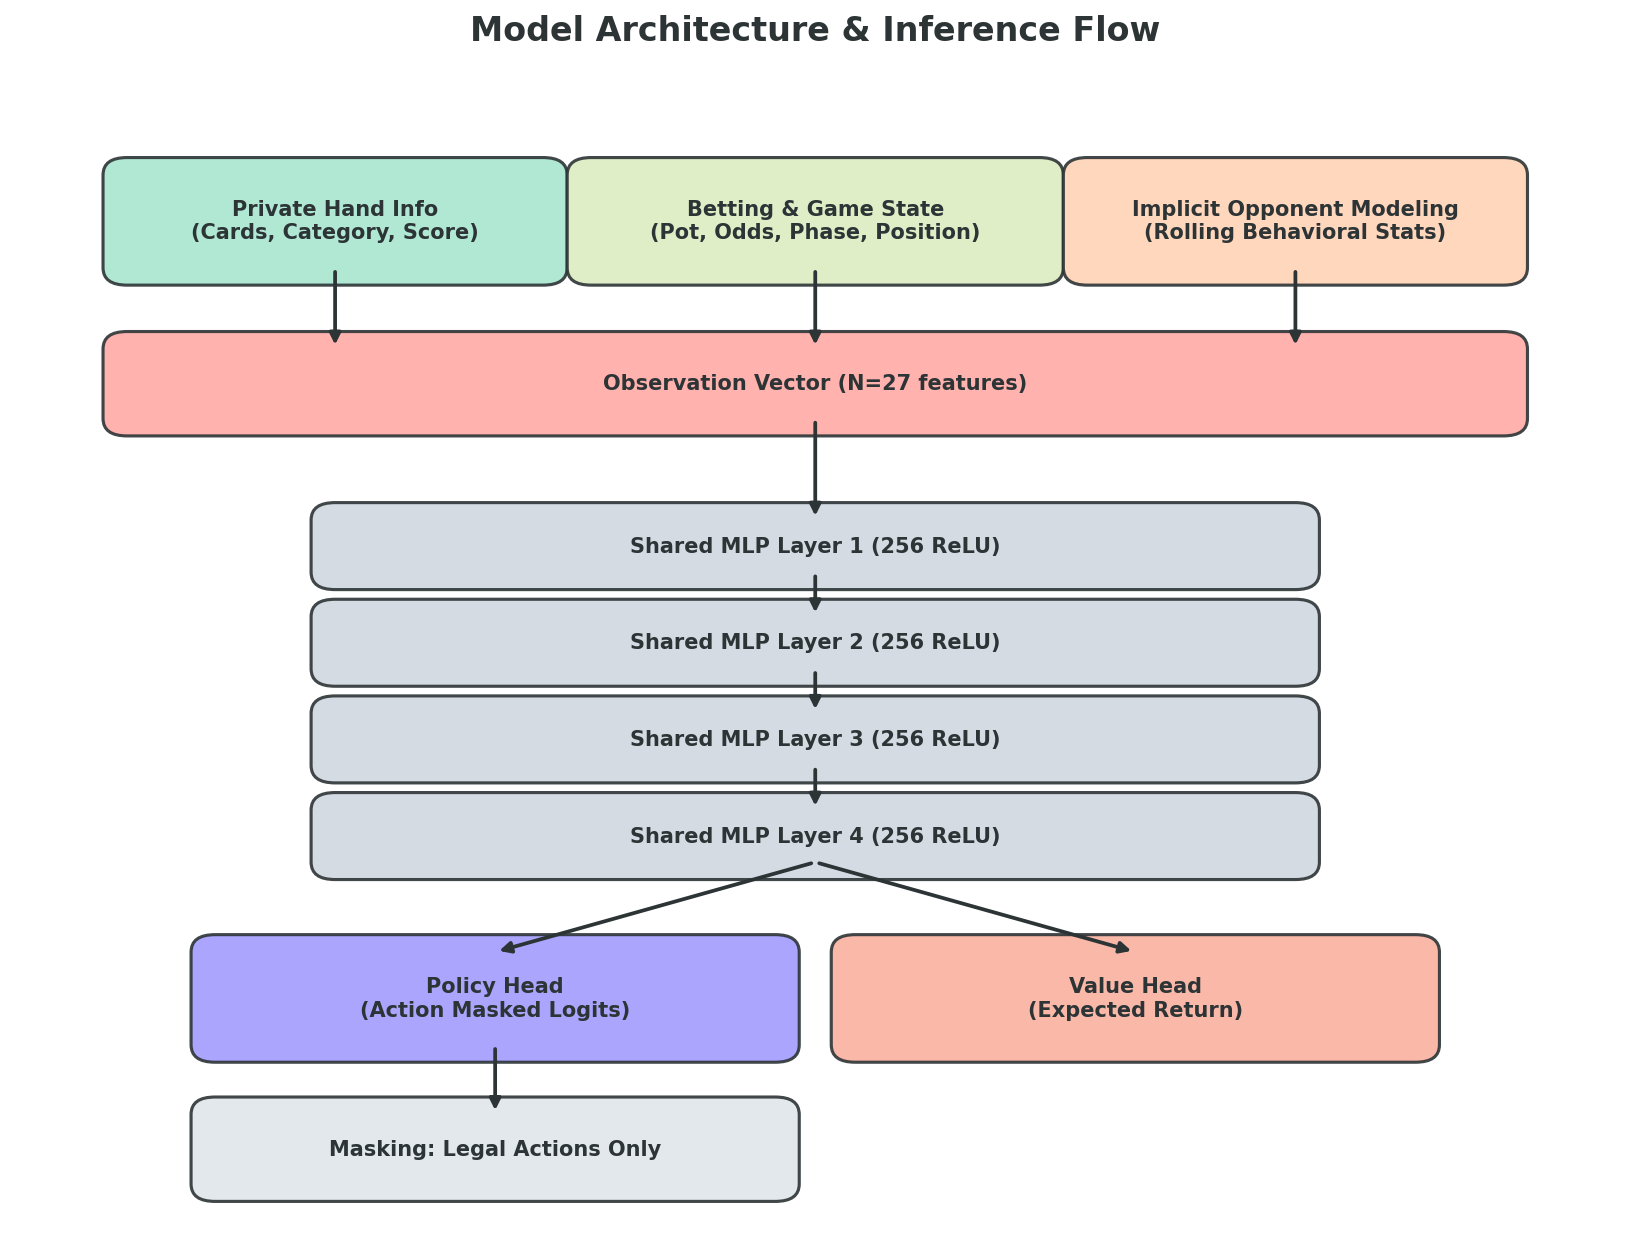
\includegraphics[width=\columnwidth]{architecture.png}
  \caption{Model~B (Implicit) architecture and inference flow. The
    observation vector concatenates private hand information, game-state
    features, and the 10-dimensional rolling behavioral statistics.
    Four shared MLP layers (256 ReLU units each) feed separate policy
    and value heads; action masking is applied before sampling.}
  \label{fig:architecture}
\end{figure}

% =====================================================================
\section{Experimental Results}
\label{sec:results}

\subsection{Cross-Evaluation Performance}

Both models are evaluated against each of the three opponent archetypes
over 10{,}000 hands, repeated across three independent evaluation seeds
(0, 100, 200). Mean BB/100 and standard deviations are reported in
Table~\ref{tab:results}. A random-action baseline is included for
reference.

\begin{table}[htbp]
\caption{Evaluation Results: BB/100 by Model and Opponent (mean $\pm$ std over 3 seeds)}
\label{tab:results}
\centering
\begin{tabular}{lccc}
\toprule
\textbf{Opponent} & \textbf{Model A (Expl.)} & \textbf{Model B (Impl.)} & \textbf{Random} \\
\midrule
CallingStation & $+86.5 \pm 4.3$ & $+79.9 \pm 5.0$ & $-143.8 \pm 2.7$ \\
Maniac         & $+408.0 \pm 15.7$ & $+390.8 \pm 11.5$ & $-222.1 \pm 0.1$ \\
Rock           & $+47.5 \pm 2.8$   & $+28.9 \pm 6.5$   & $-151.3 \pm 2.0$ \\
\midrule
\textbf{Average} & $+180.65$ & $+166.50$ & $-172.44$ \\
\bottomrule
\end{tabular}
\end{table}

Both trained agents substantially outperform the random baseline across
all archetypes. Model~A (Explicit) posts the higher average (+180.65 BB/100
vs.\ +166.50 BB/100 for Model~B), which is expected given that it receives
the opponent identity directly in its observation. The gap is most
pronounced against the Rock archetype (+47.5 vs.\ +28.9), a hard-to-exploit
opponent that only invests chips with strong holdings. Against the Maniac,
both models achieve very high profitability, as the Maniac's loose
aggression and frequent draws create many exploitable spots.

Fig.~\ref{fig:bb_comparison} shows the cross-evaluation profitability as a
grouped bar chart, and Fig.~\ref{fig:cumulative} shows cumulative profit
trajectories over 30{,}000 hands (three seeds concatenated). The linear
growth of the profit curves for both trained agents confirms that their
exploitative advantage is stable and does not degrade over longer horizons.

\begin{figure}[htbp]
  \centering
  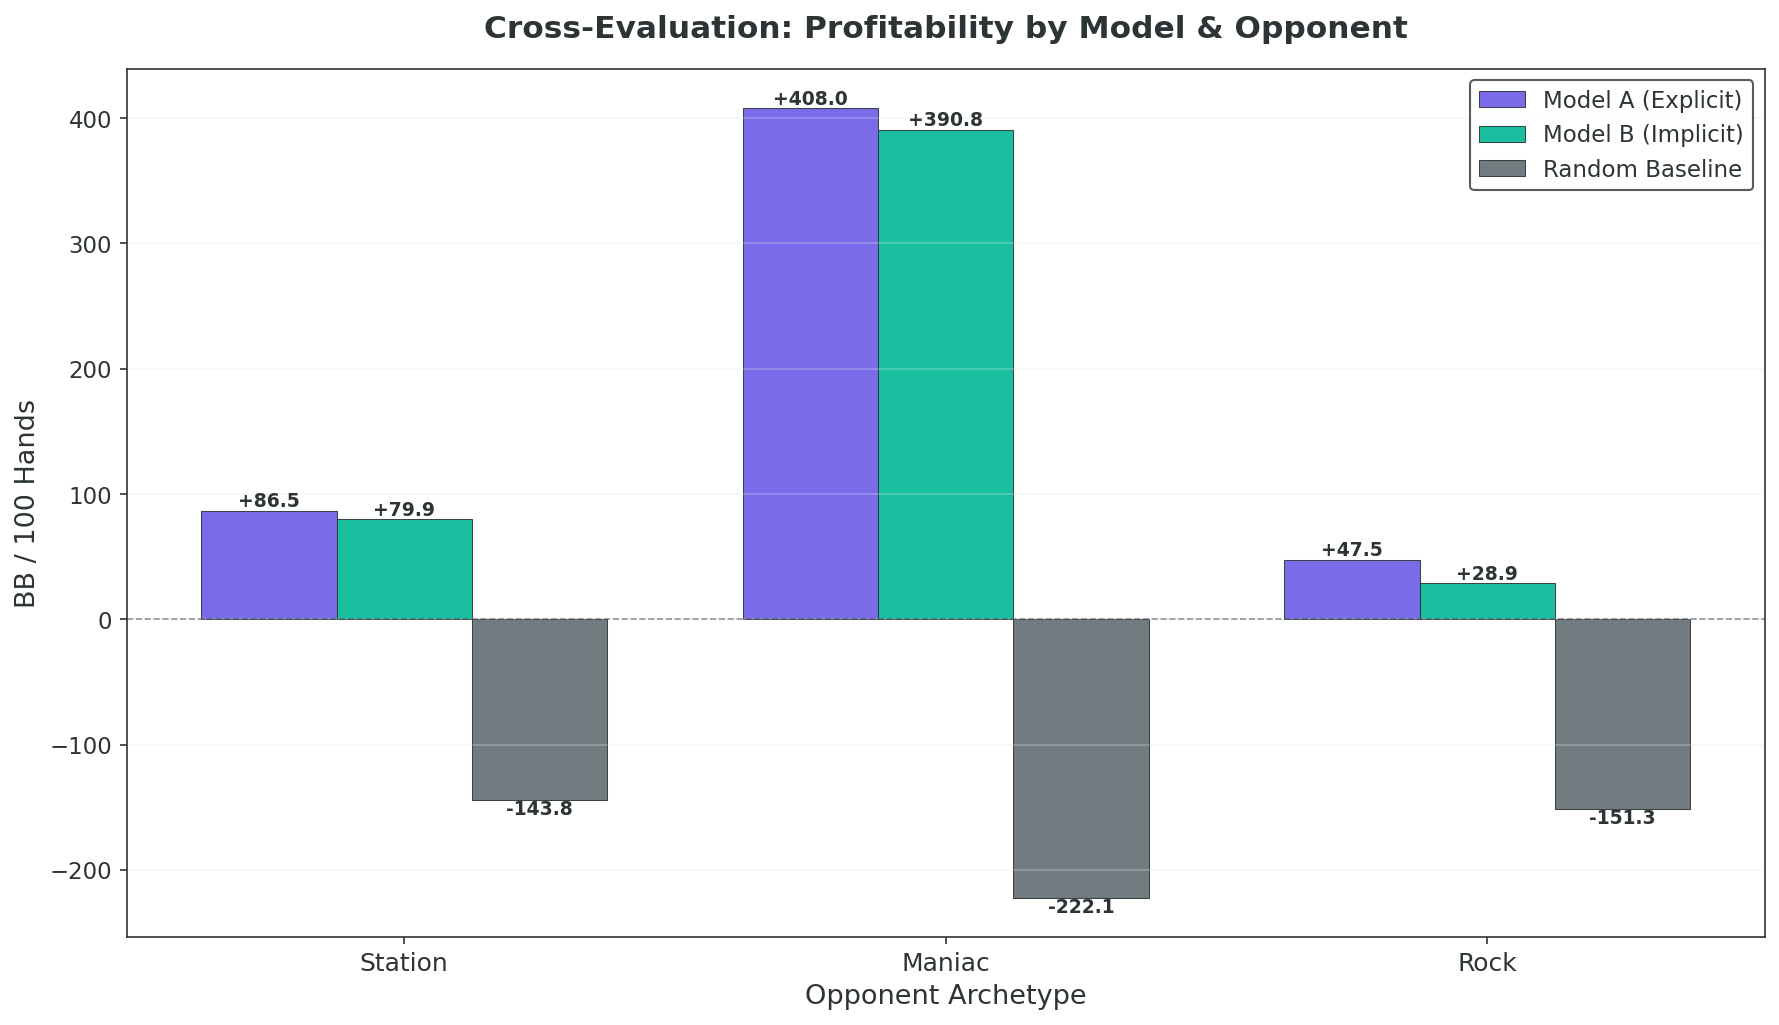
\includegraphics[width=\columnwidth]{bb_per_100_comparison.png}
  \caption{Cross-evaluation profitability (BB/100) for Model~A (Explicit),
    Model~B (Implicit), and the random baseline across the three opponent
    archetypes. Error bars are not shown in the bar chart but are provided
    in Table~\ref{tab:results}.}
  \label{fig:bb_comparison}
\end{figure}

\begin{figure*}[htbp]
  \centering
  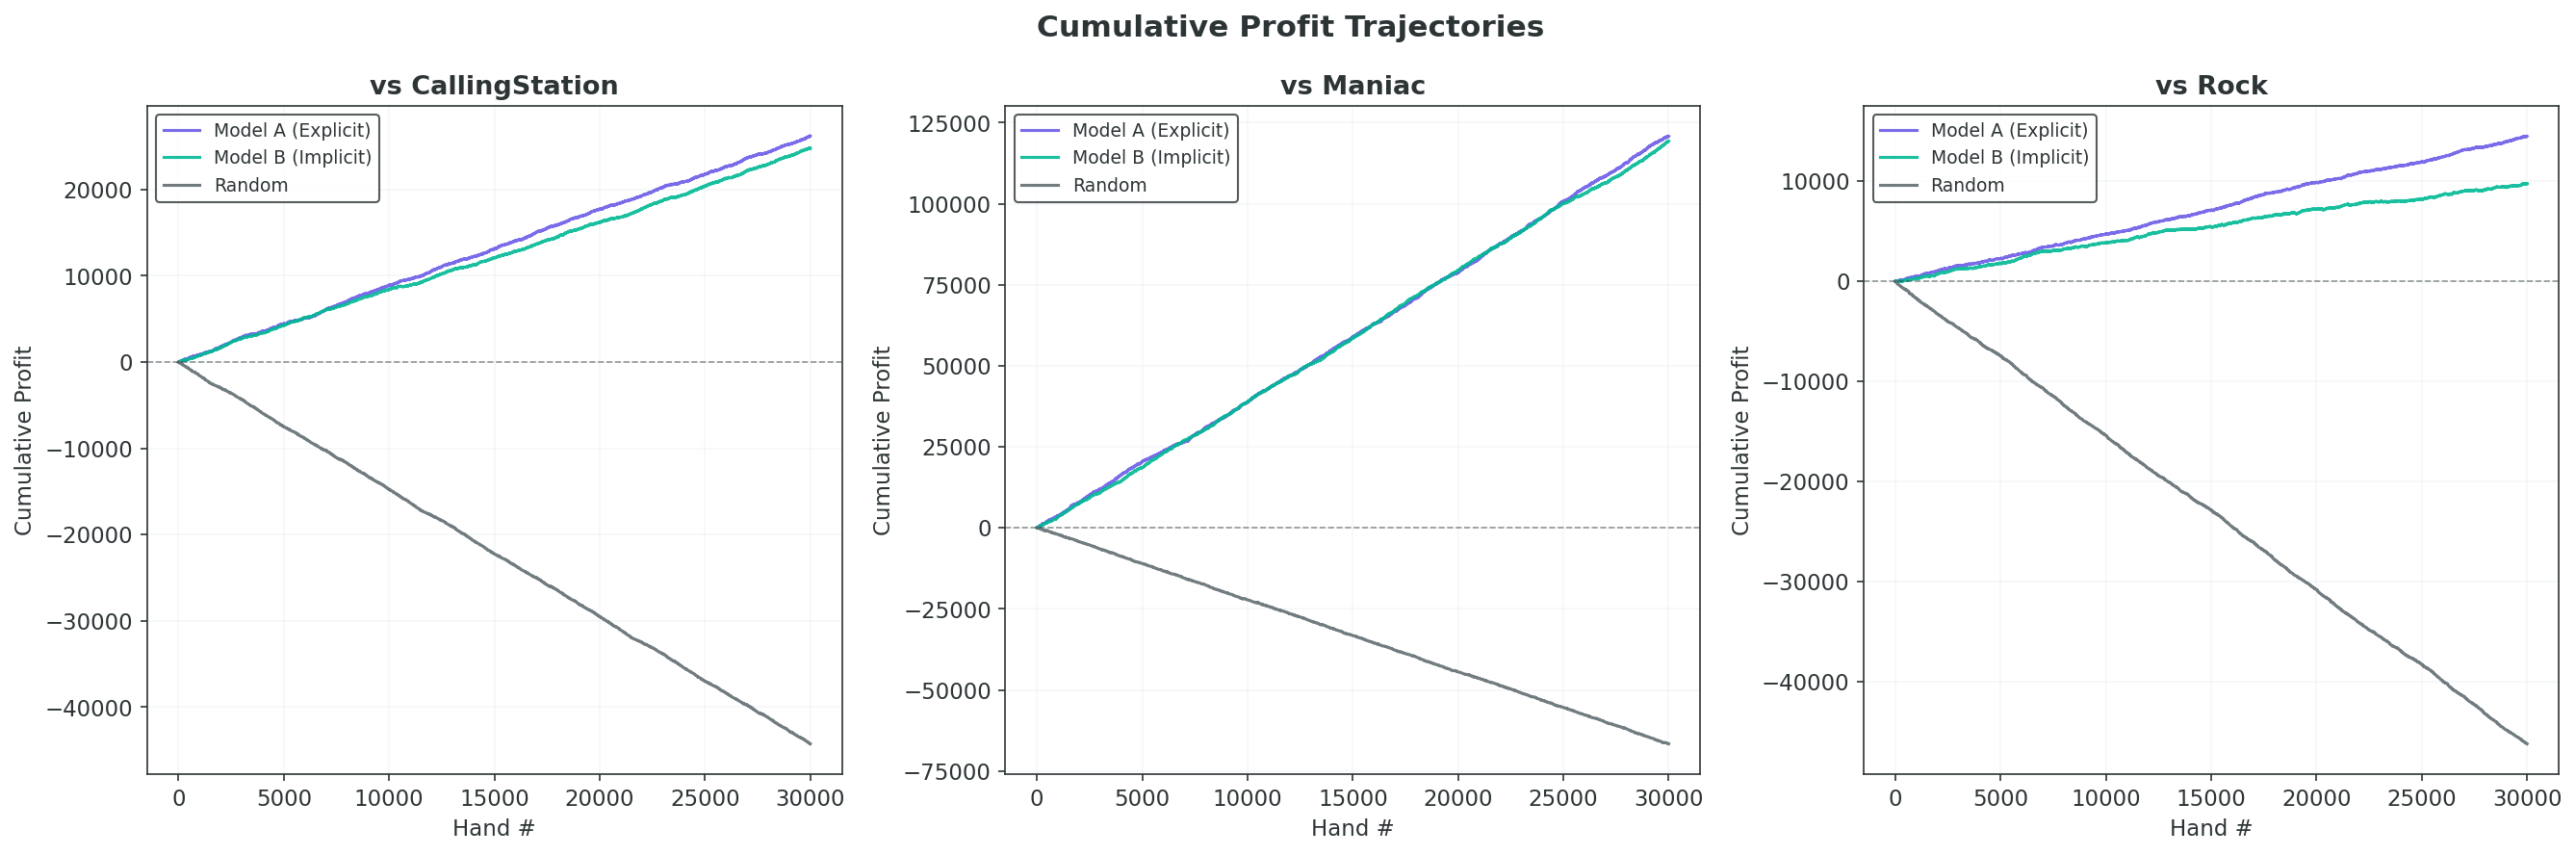
\includegraphics[width=\textwidth]{cumulative_profit.png}
  \caption{Cumulative profit trajectories over 30{,}000 hands (three
    10{,}000-hand evaluation seeds concatenated) per opponent archetype.
    Both trained models exhibit consistent positive linear growth,
    while the random baseline degrades uniformly.}
  \label{fig:cumulative}
\end{figure*}

\subsection{Behavioral Analysis: ``The Tell''}

A central contribution of this work is the behavioral matrix analysis of
Model~B's post-draw action distribution, conditioned on the observed
opponent draw count. Fig.~\ref{fig:behavioral} displays the frequency
of Fold, Call, and Raise actions for three representative draw-count
values (0, 1, and 3) across each opponent archetype.

\begin{figure*}[htbp]
  \centering
  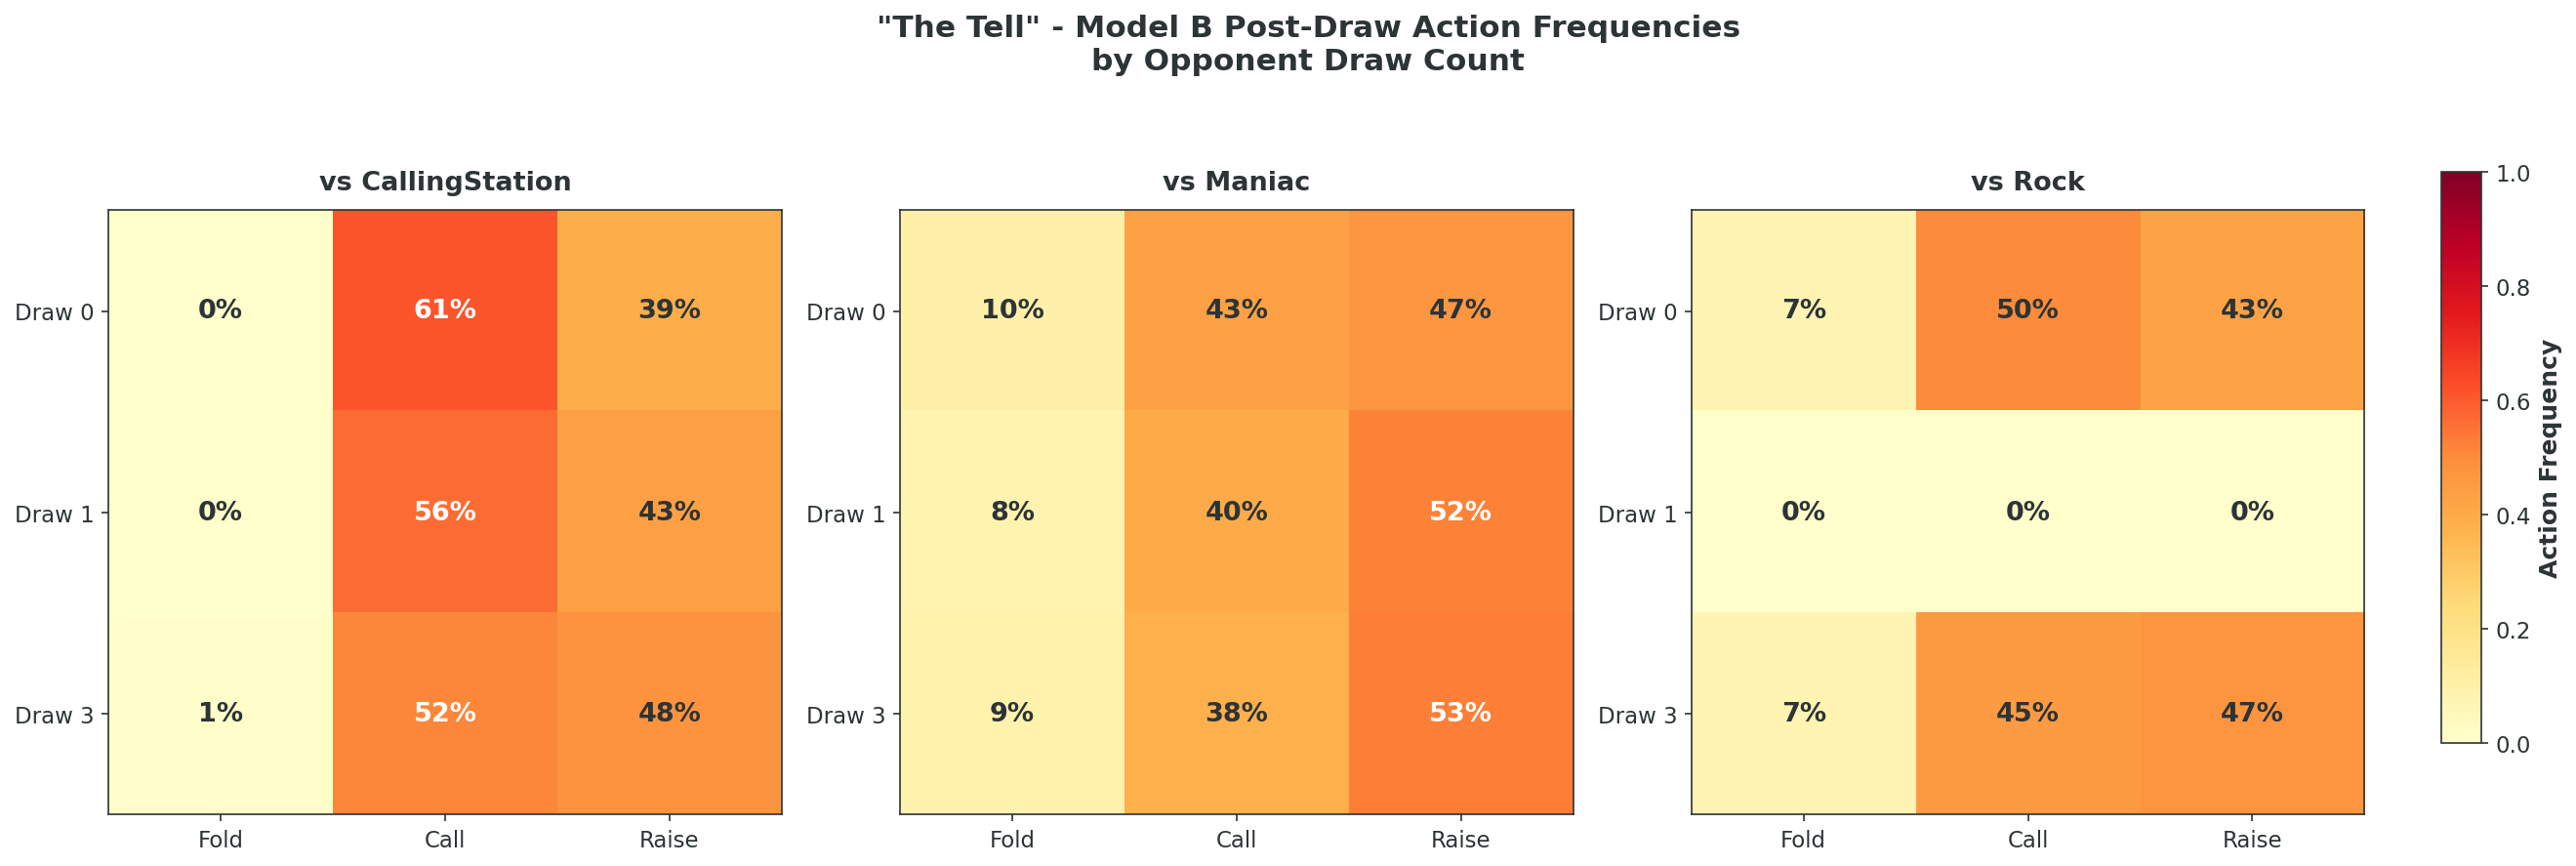
\includegraphics[width=\textwidth]{behavioral_matrix.png}
  \caption{``The Tell'': Model~B post-draw action frequencies conditioned on
    opponent draw count (rows) for each opponent archetype (panels). Model~B
    adapts its post-draw aggression based on opponent draw count without
    access to explicit opponent identity.}
  \label{fig:behavioral}
\end{figure*}

Several patterns emerge from the matrix. Against the CallingStation,
Model~B maintains consistently high call and raise frequencies regardless
of draw count (0\% fold rate when the station stands pat or draws one),
reflecting the station's predictably passive post-draw behavior. Against
the Maniac, the model increases its raise frequency when the Maniac draws
one card (52\%), as a single-card draw from a loose opponent is a common
flush or straight chase that frequently misses. The most striking pattern
appears against the Rock: when the Rock stands pat (Draw~0), Model~B
responds with 50\% call and 43\% raise, treating a Rock stand-pat as a
strong hand signal. When the Rock draws one card, Model~B's call and raise
frequencies drop to 0\%, indicating learned recognition that this is an
unusual Rock action associated with high hand strength. These patterns
demonstrate that Model~B has learned opponent-specific hand-reading
heuristics from draw-count telemetry alone, without any explicit archetype
identifier in its input.

\subsection{Non-Stationary Adaptation}

To evaluate Model~B's ability to adapt when the opponent changes mid-session,
we run a 1{,}500-hand tournament in which the opponent switches from
CallingStation (hands 1--500) to Maniac (hands 501--1{,}000) to Rock
(hands 1{,}001--1{,}500) without resetting Model~B's rolling statistics buffer.
Two variants of Model~A are also evaluated: an \textit{Oracle} variant given
the correct archetype label at each switch, and a \textit{Blind} variant
given a fixed incorrect label throughout.

\begin{figure*}[htbp]
  \centering
  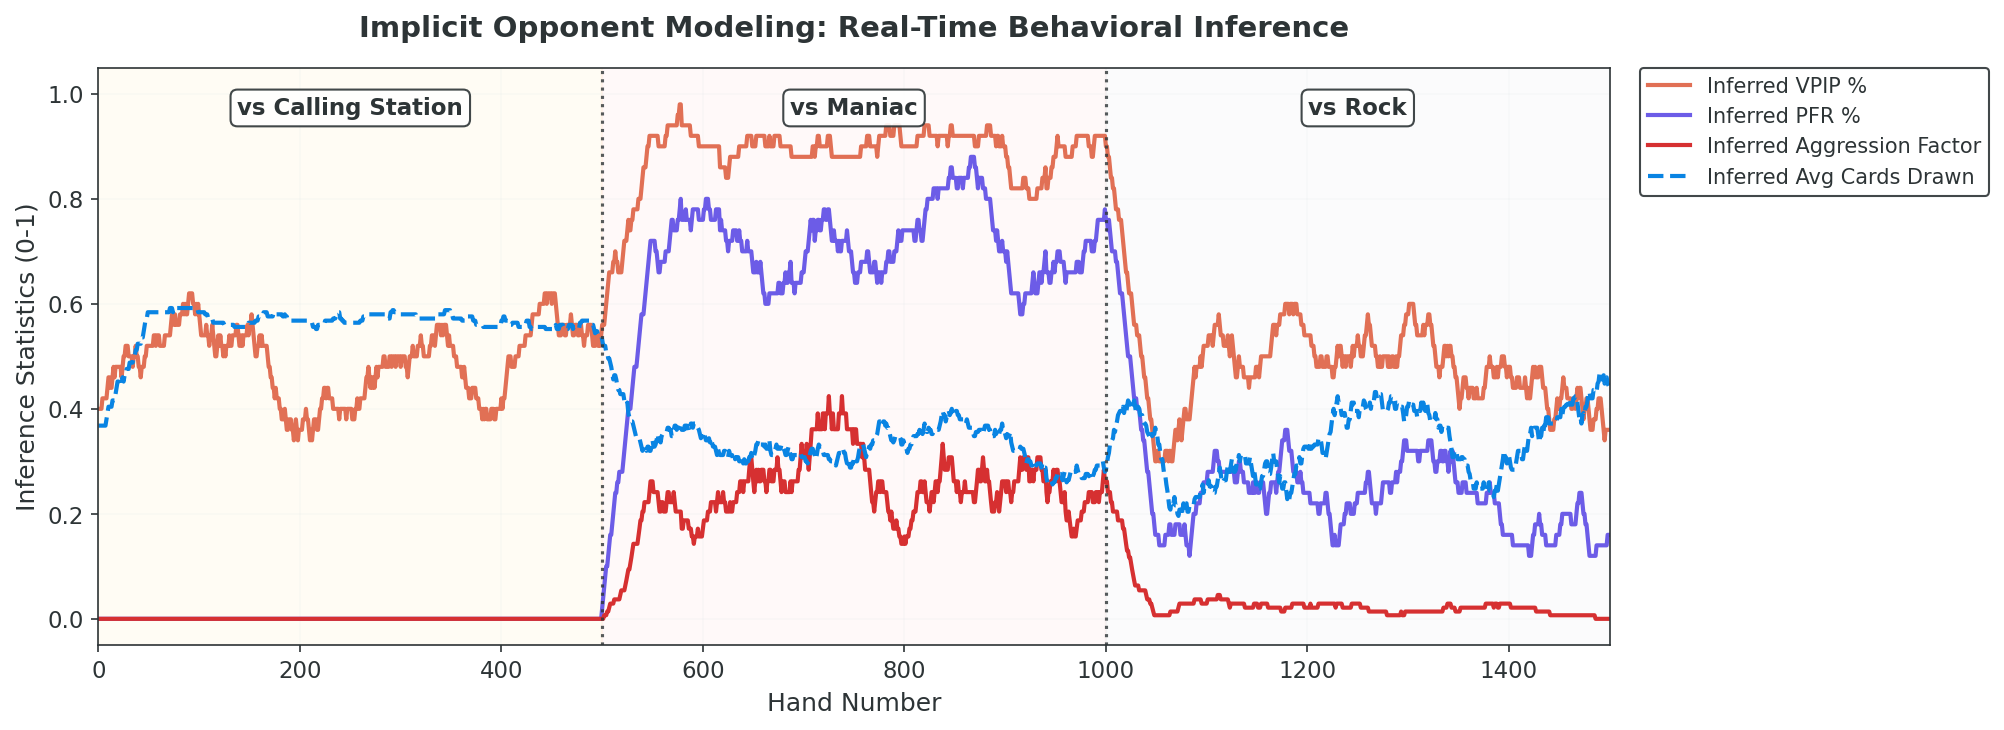
\includegraphics[width=\textwidth]{non_stationary_inference.png}
  \caption{Model~B's rolling behavioral statistics (VPIP, PFR, Aggression
    Factor, Avg.\ Cards Drawn) across the 1{,}500-hand non-stationary
    tournament. Vertical dashed lines mark opponent switches. The statistics
    adapt within $\sim$50--100 hands after each switch.}
  \label{fig:ns_inference}
\end{figure*}

\begin{figure*}[htbp]
  \centering
  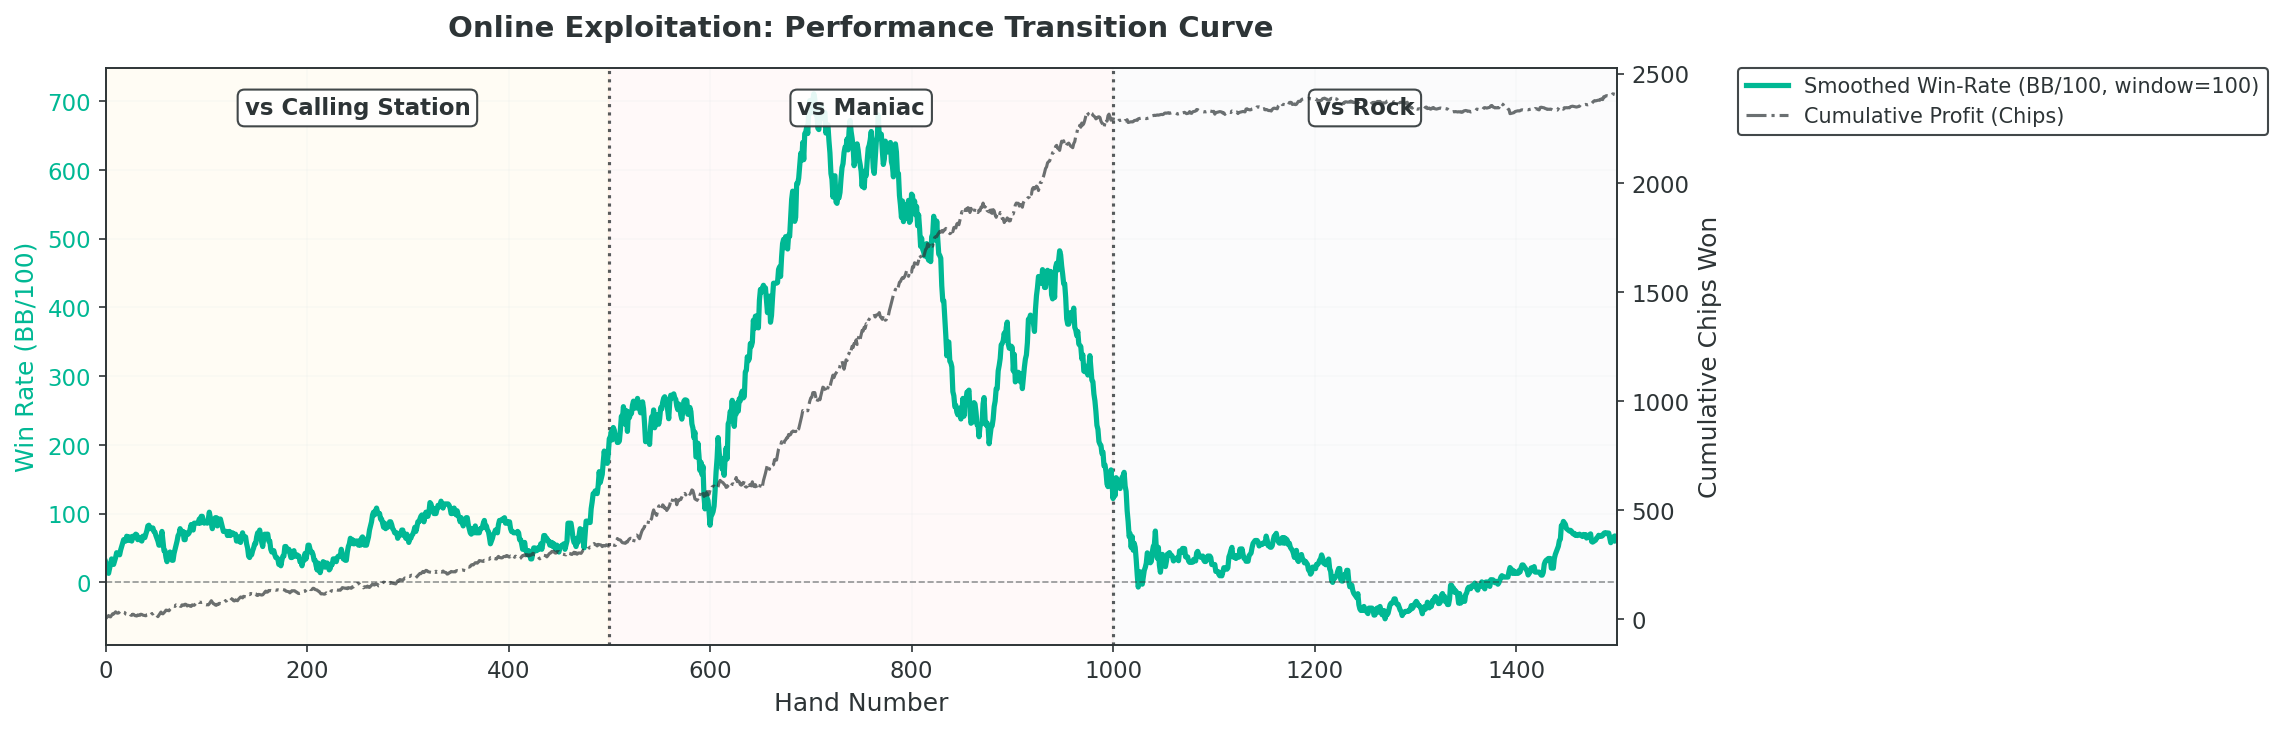
\includegraphics[width=\textwidth]{non_stationary_performance.png}
  \caption{Online exploitation performance of Model~B in the non-stationary
    tournament: smoothed win rate (BB/100, window=100) and cumulative profit.
    Win rate peaks during the Maniac segment and recovers after each opponent
    switch with a brief transient.}
  \label{fig:ns_performance}
\end{figure*}

Results of the tournament are summarized in Table~\ref{tab:nonstationary}.
Model~B achieves +160.35 BB/100, outperforming Model~A-Oracle (+156.28
BB/100) and substantially outperforming Model~A-Blind (+50.01 BB/100).
Fig.~\ref{fig:ns_inference} shows that the rolling statistics
(VPIP, PFR, Aggression Factor, Avg.\ Cards Drawn) adapt to the new
opponent within approximately 50--100 hands after each switch.
Fig.~\ref{fig:ns_performance} shows the corresponding win-rate curve, with
brief transients at each switch point followed by recovery.

\begin{table}[htbp]
\caption{Non-Stationary Adaptation Tournament Results (1,500 hands)}
\label{tab:nonstationary}
\centering
\begin{tabular}{lc}
\toprule
\textbf{Agent} & \textbf{BB/100} \\
\midrule
Model B (Implicit)          & $+160.35$ \\
Model A (Explicit -- Oracle) & $+156.28$ \\
Model A (Explicit -- Blind)  & $+50.01$  \\
\bottomrule
\end{tabular}
\end{table}

\subsection{Statistical Validation}

Statistical significance of Model~B's performance is assessed over
270{,}000 pooled hands (three opponents $\times$ three seeds $\times$
10{,}000 hands each). A paired $t$-test comparing per-hand profit between
Model~B and Model~A yields $t = -2.183$, $p = 0.029$, indicating that
the difference in means is statistically significant at the $\alpha = 0.05$
level. Model~B vs.\ the random baseline is highly significant ($t = +106.85$,
$p \approx 0$). A 95\% confidence interval for Model~B's average per-hand
profit gives $+1.71$ chips [CI: 1.65, 1.76], corresponding to $+170.87$
BB/100 [CI: 165.31, 176.44].

% =====================================================================
\section{Discussion}
\label{sec:discussion}

\subsection{Implicit vs.\ Explicit Modeling}

The performance gap between Model~A and Model~B---roughly 14 BB/100 on
average---is consistent with the information asymmetry: Model~A receives
the opponent archetype as a direct input, while Model~B must infer it from
behavioral evidence accumulated over recent hands. The gap is largest against
the Rock (+18.6 BB/100 in favor of Model~A), whose tight-passive style
generates sparse exploitable signals. Against the Maniac, the gap narrows
considerably (+17.2 BB/100), suggesting that the Maniac's high VPIP and
frequent draws are sufficient to produce a strong implicit signal within the
rolling window of $W=50$ hands.

\subsection{The Non-Stationary Advantage}

Somewhat counterintuitively, Model~B slightly outperforms Model~A-Oracle in
the non-stationary tournament (+160.35 vs.\ +156.28 BB/100). One plausible
explanation is that Model~B's rolling statistics provide a more nuanced,
\textit{continuous} representation of opponent behavior than a single one-hot
identity label. When the opponent plays a mix of strategies at the boundary
of archetype definitions, the rolling statistics can capture subtle
intermediate states that the discrete label cannot. This interpretation
aligns with the behavioral matrix in Fig.~\ref{fig:behavioral}, which shows
that Model~B conditions on draw-count in an archetype-specific manner.

\subsection{Limitations}

Several limitations bound the scope of our conclusions. First, all opponents
are hand-coded deterministic or fixed-stochastic archetypes; the agent has
not been tested against adaptive or self-play opponents. Second, the training
environment uses limit betting with a fixed ante, which removes no-limit
strategic considerations such as stack-size-aware bet-sizing. Third, the
rolling statistics window size ($W=50$) requires several dozen hands before
the behavioral signal stabilizes, which imposes a cold-start cost when the
opponent switches. Finally, the evaluation is restricted to heads-up play;
generalization to multi-player settings would require significant
architectural changes.

% =====================================================================
\section{Conclusion}
\label{sec:conclusion}

We presented CardShark-RL, a reinforcement learning system for heads-up
5-Card Draw Poker that investigates two approaches to opponent adaptation.
Model~A uses explicit opponent identity to condition its policy, while
Model~B infers opponent behavior from a rolling window of behavioral
statistics. Both models substantially outperform a random baseline across
all tested archetypes. Model~B achieves an average of +166.50 BB/100,
compared to +180.65 BB/100 for Model~A, with the gap being statistically
significant ($p = 0.029$) but practically modest given that Model~B has
no access to opponent identity.

The behavioral matrix analysis reveals that Model~B has learned
opponent-specific hand-reading heuristics from draw-count telemetry alone.
In the non-stationary tournament, Model~B marginally outperforms
Model~A-Oracle (+160.35 vs.\ +156.28 BB/100), indicating that implicit
behavioral inference can be more robust than explicit labeling when the
environment is non-stationary.

Future work could extend this framework to no-limit betting, self-play
training, and multi-player settings. Incorporating uncertainty estimates
over the opponent's hand range---combining the implicit behavioral
statistics with Bayesian hand-range inference---could further narrow the
gap with explicit modeling, particularly against tight-passive opponents
like the Rock.

% =====================================================================
\section*{Acknowledgment}
The authors thank the Department of Computer Engineering at Izmir
Katip Celebi University for providing computational resources and
course infrastructure.

% =====================================================================
\bibliographystyle{IEEEtran}
\bibliography{references}

\end{document}
